\documentclass[UTF8,a4paper,zihao=5]{ctexart}

\usepackage{amsmath,amssymb,bm}
\usepackage{booktabs}
\usepackage{graphicx}
\usepackage{geometry}
\usepackage{siunitx}
\usepackage{caption}
\usepackage{subcaption}
\usepackage{float}
\usepackage{hyperref}

\geometry{left=2.8cm,right=2.8cm,top=2.6cm,bottom=2.6cm}
\hypersetup{colorlinks=true,linkcolor=black,citecolor=black,urlcolor=black}
\sisetup{detect-all}
\setcounter{tocdepth}{2}
\renewcommand{\topfraction}{0.9}
\renewcommand{\bottomfraction}{0.8}
\renewcommand{\textfraction}{0.08}
\renewcommand{\floatpagefraction}{0.85}

\title{\bfseries 悬臂梁式简易电子秤的设计、制作与标定}
\author{
  姓名：\underline{\hspace{3cm}}
  \quad 学号：\underline{\hspace{3cm}}
  \quad 班级：\underline{\hspace{3cm}}
}
\date{\today}

\begin{document}

\newgeometry{left=1.95cm,right=1.95cm,top=0.65cm,bottom=0.75cm}
\begin{titlepage}
\thispagestyle{empty}
\newcommand{\coverfield}[2]{%
  \makebox[3.35cm][l]{#1}%
  \underline{\makebox[10.4cm][c]{#2}}}
\newcommand{\memberfield}[3]{%
  \makebox[3.35cm][l]{#1}%
  \underline{\makebox[5.25cm][c]{#2}}%
  \hspace{0.45cm}（\underline{\makebox[3.4cm][c]{#3}}）}

{\setlength{\unitlength}{1mm}
\begin{picture}(0,0)
  \put(136.5,-1.0){\line(1,0){34.5}}
  \put(136.5,-11.5){\line(1,0){34.5}}
  \put(136.5,-36.0){\line(1,0){34.5}}
  \put(136.5,-1.0){\line(0,-1){35.0}}
  \put(171.0,-1.0){\line(0,-1){35.0}}
  \put(136.5,-10.2){\makebox(34.5,8)[c]{\zihao{3}\bfseries 成\quad 绩}}
\end{picture}}

\vspace*{1.65cm}
\noindent\makebox[\textwidth][c]{%
  
\includegraphics[width=7.2cm,trim=8bp 4bp 0bp 0bp,clip]{figures/浙大标志.png}}

\vspace{1.28cm}
\begin{center}
{\zihao{3}\bfseries
\setlength{\baselineskip}{1.45cm}
\coverfield{课程名称：}{材\quad 料\quad 力\quad 学\quad 实\quad 验}\par
\coverfield{实验选题：}{悬臂梁式简易电子秤的设计、制作与标定}\par
\coverfield{指导老师：}{雷华}\par
\coverfield{选课班级：}{2026\quad 夏\quad 周一6.7节}\par
\memberfield{团队成员：}{韩颂义}{3240104198}\par
\memberfield{}{姚珂尔}{3240103616}\par
\memberfield{}{张雨童}{3240100241}\par
}
\end{center}
\vfill
\begin{center}
  
\includegraphics[width=9.0cm]{figures/最下面.png}
\end{center}
\end{titlepage}
\restoregeometry

\pagenumbering{Roman}
\setcounter{page}{1}

\begin{abstract}
本文围绕悬臂梁式简易电子秤的设计与标定展开研究。以弹簧钢
40CrNiMoA 梁作为弹性元件，基于材料力学中悬臂梁弯曲应力与应变关系，
确定应变片布置方案、惠斯登电桥组桥方式、信号放大方案，并对弹性元件
进行强度校核和量程设计。通过加载标定实验建立输出电压与质量之间的线性关系，
进一步评价电子秤的灵敏度、线性度、重复性、精度等级和有效量程。最后结合
固定端影响、贴片位置误差、偏心加载、温度漂移、电路非线性等因素进行误差分析，
给出改进方案。
\end{abstract}

\noindent\textbf{关键词：}悬臂梁；应变片；惠斯登电桥；电子秤；强度校核；标定

\clearpage
\begingroup
\normalsize
\linespread{1.18}\selectfont
\setlength{\parskip}{0.18em}
\makeatletter
\renewcommand*\l@section{\@dottedtocline{1}{0em}{2.8em}}
\renewcommand*\l@subsection{\@dottedtocline{2}{1.8em}{3.5em}}
\makeatother
\tableofcontents
\endgroup
\clearpage
\pagenumbering{arabic}
\setcounter{page}{1}

\section{引言}

\subsection{实验背景}

电子秤是力学量测量与工程检测中常见的传感装置，其核心是将外加载荷转化为
可测量的电信号。应变片式传感器利用电阻应变效应工作，具有结构简单、灵敏度
较高、易于组桥和便于信号放大的特点。本实验以矩形截面悬臂梁作为弹性元件，
通过分析梁在集中载荷作用下的弯曲应变，建立质量与电桥输出之间的对应关系，
从而完成简易电子秤的设计、制作与标定。

\subsection{实验目的}

\begin{enumerate}
  \item 设计一种结果不受固定位置和加载位置显著影响的悬臂梁式简易电子秤；
  \item 对弹性元件进行受力分析和强度校核，确定安全量程；
  \item 确定应变片贴片位置、组桥方式；
  \item 通过标定实验建立质量与输出信号的关系；
  \item 分析实验误差，确定电子秤的精度等级和有效量程。
\end{enumerate}

\section{实验对象与基本参数}

\subsection{弹性元件几何与材料参数}

本实验采用矩形截面悬臂梁作为弹性元件。实验梁长
\(L_0=\SI{450}{mm}\)，截面宽度 \(b=\SI{30}{mm}\)，厚度
\(t=\SI{4}{mm}\)。材料为弹簧钢 40CrNiMoA，屈服强度取
\(\sigma_{0.2}=\SI{980}{MPa}\)，弹性模量取
\(E=\SI{210}{GPa}\)。

实际装夹后，固定端到挂载位置之间的有效力臂为
\(L_1=\SI{320}{mm}\)。因此，涉及弯矩、应力和量程估算的计算均采用
\(L_1\)，而梁总长 \(L_0\) 仅作为弹性元件的几何尺寸参数。

矩形截面对受弯方向的惯性矩和抗弯截面系数可写为
\begin{equation}
  I=\frac{bt^3}{12}, \qquad W=\frac{I}{t/2}=\frac{bt^2}{6}.
  \label{eq:section-modulus}
\end{equation}

\subsection{符号说明}

\begin{table}[H]
  \centering
  \small
  \setlength{\tabcolsep}{3pt}
  \renewcommand{\arraystretch}{0.92}
  \begin{tabular}{c>{\raggedright\arraybackslash}p{3.8cm}cc>{\raggedright\arraybackslash}p{3.8cm}c}
    \toprule
    符号 & 含义 & 单位 & 符号 & 含义 & 单位 \\
    \midrule
    \(P\) & 作用在悬臂梁上的集中载荷 & N
    & \(W\) & 抗弯截面系数 & mm\(^3\) \\
    \(m\) & 被测物体质量 & kg
    & \(M\) & 截面弯矩 & N\(\cdot\)mm \\
    \(L_1\) & 固定端到挂载位置的有效力臂 & mm
    & \(\sigma\) & 弯曲正应力 & MPa \\
    \(x\) & 应变片位置到固定端的距离 & mm
    & \(\varepsilon\) & 梁表面应变 & -- \\
    \(E\) & 材料弹性模量 & MPa
    & \(K\) & 应变片灵敏度系数 & -- \\
    \bottomrule
  \end{tabular}
  \caption{主要符号说明}
\end{table}

\section{理论分析}

\subsection{悬臂梁受力与弯矩分析}

当载荷 \(P=mg\) 作用于距固定端 \(a\) 处时，距固定端 \(x\) 处截面的弯矩为
\begin{equation}
  M(x)=P(a-x), \qquad 0\leq x\leq a.
  \label{eq:bending-moment}
\end{equation}
本实验中载荷作用点为挂载位置，因此在后续具体计算中取
\(a=L_1=\SI{320}{mm}\)。

梁表面最大弯曲应力为
\begin{equation}
  \sigma(x)=\frac{M(x)}{W}.
  \label{eq:bending-stress}
\end{equation}

由胡克定律可得
\begin{equation}
  \sigma=E\varepsilon,
  \qquad
  \varepsilon(x)=\frac{P(a-x)}{EW}.
  \label{eq:strain-load}
\end{equation}

若在两个不同位置 \(x_1,x_2\) 处布置应变片，则可由弯矩差估计剪力：
\begin{equation}
  Q=\frac{dM}{dx}\approx \frac{M_2-M_1}{x_2-x_1}.
  \label{eq:shear-force}
\end{equation}
在悬臂梁集中力加载条件下，剪力与载荷大小相等。因此，通过差动测量不同截面
的弯矩或应变，有望减弱加载点位置变化对测量结果的影响。

\subsection{应变片电阻变化与电桥输出}

金属电阻应变片的相对电阻变化与应变近似满足
\begin{equation}
  \frac{\Delta R}{R}=K\varepsilon,
  \label{eq:gauge-factor}
\end{equation}
其中 \(K\) 为应变片灵敏度系数。

采用惠斯登电桥进行测量时，若四臂均为工作应变片并按拉压相反方向接入，
其基本桥路如图~\ref{fig:wheatstone-bridge} 所示。理想小变形条件下输出可近似写为
\begin{figure}[H]
  \centering
  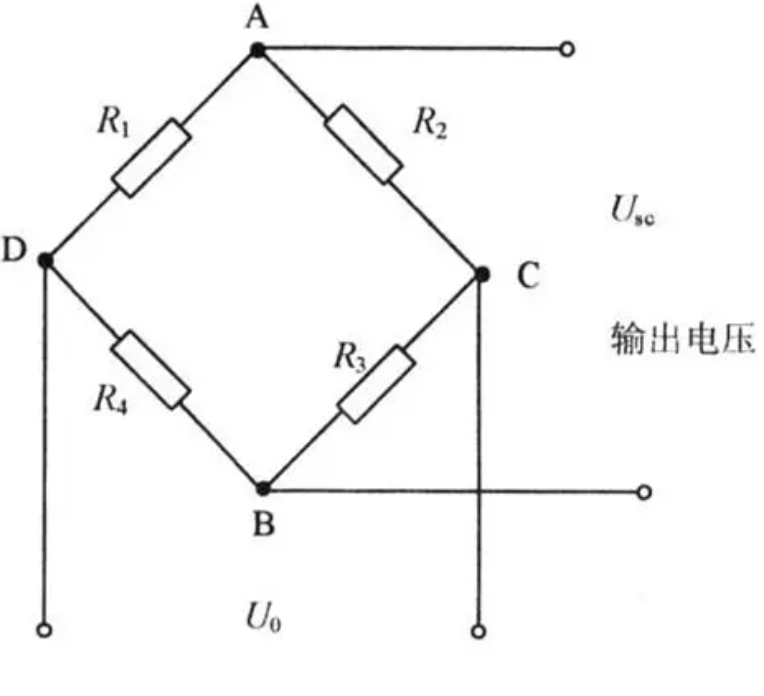
\includegraphics[width=0.52\textwidth]{figures/惠斯登电桥.png}
  \caption{惠斯登电桥基本结构示意图}
  \label{fig:wheatstone-bridge}
\end{figure}

\begin{equation}
  \frac{U_o}{U_i}
  =\frac{1}{4}K(\varepsilon_1-\varepsilon_2+\varepsilon_3-\varepsilon_4).
  \label{eq:bridge-output}
\end{equation}

本实验采用全桥接线方式，具体接线方案见下文。

\section{电子秤设计方案}

\subsection{总体结构}

本装置由弹性元件、应变片、应变仪（内置惠斯登电桥）和载物平台组成。

\begin{figure}[H]
  \centering
  \begin{subfigure}[b]{0.38\textwidth}
    \centering
    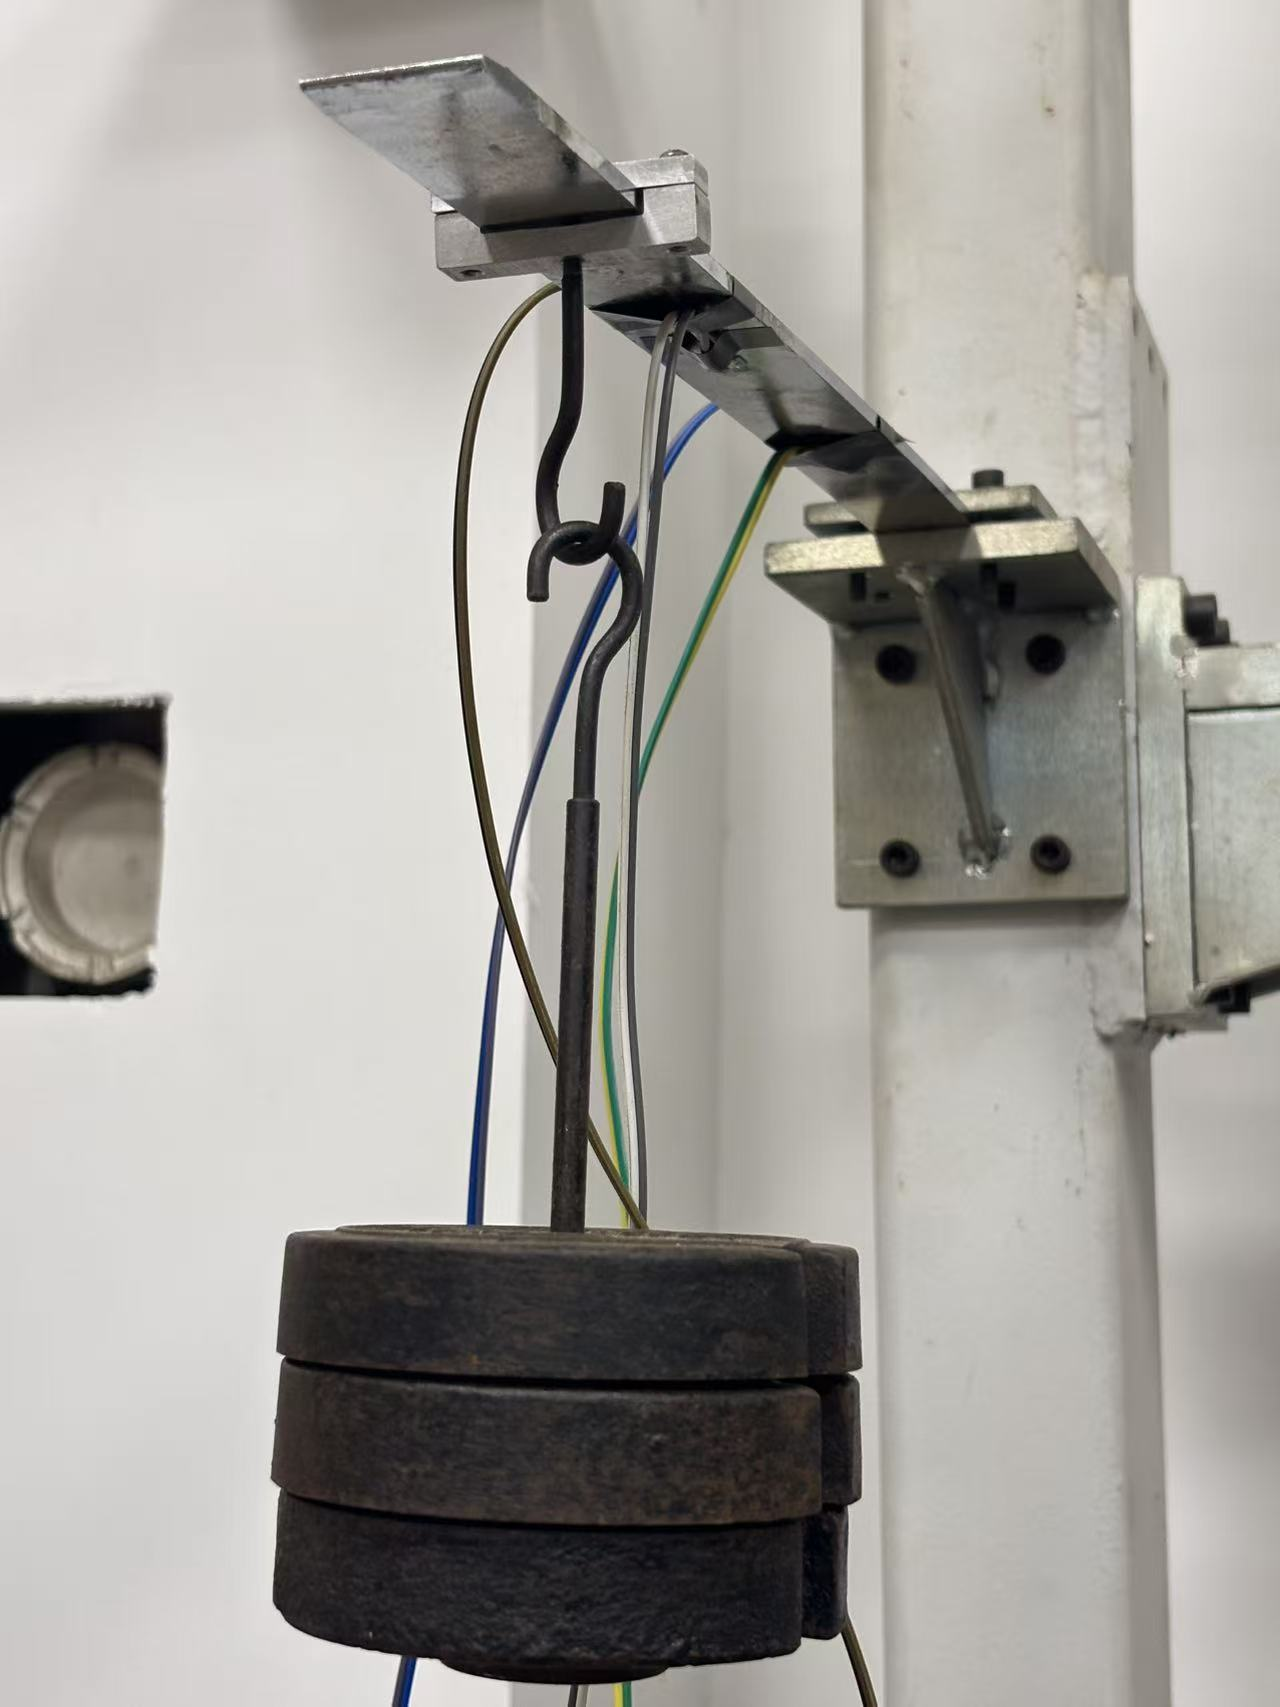
\includegraphics[height=5.2cm]{figures/载物平台.jpg}
    \caption{载物平台}
    \label{fig:loading-platform}
  \end{subfigure}
  \hfill
  \begin{subfigure}[b]{0.55\textwidth}
    \centering
    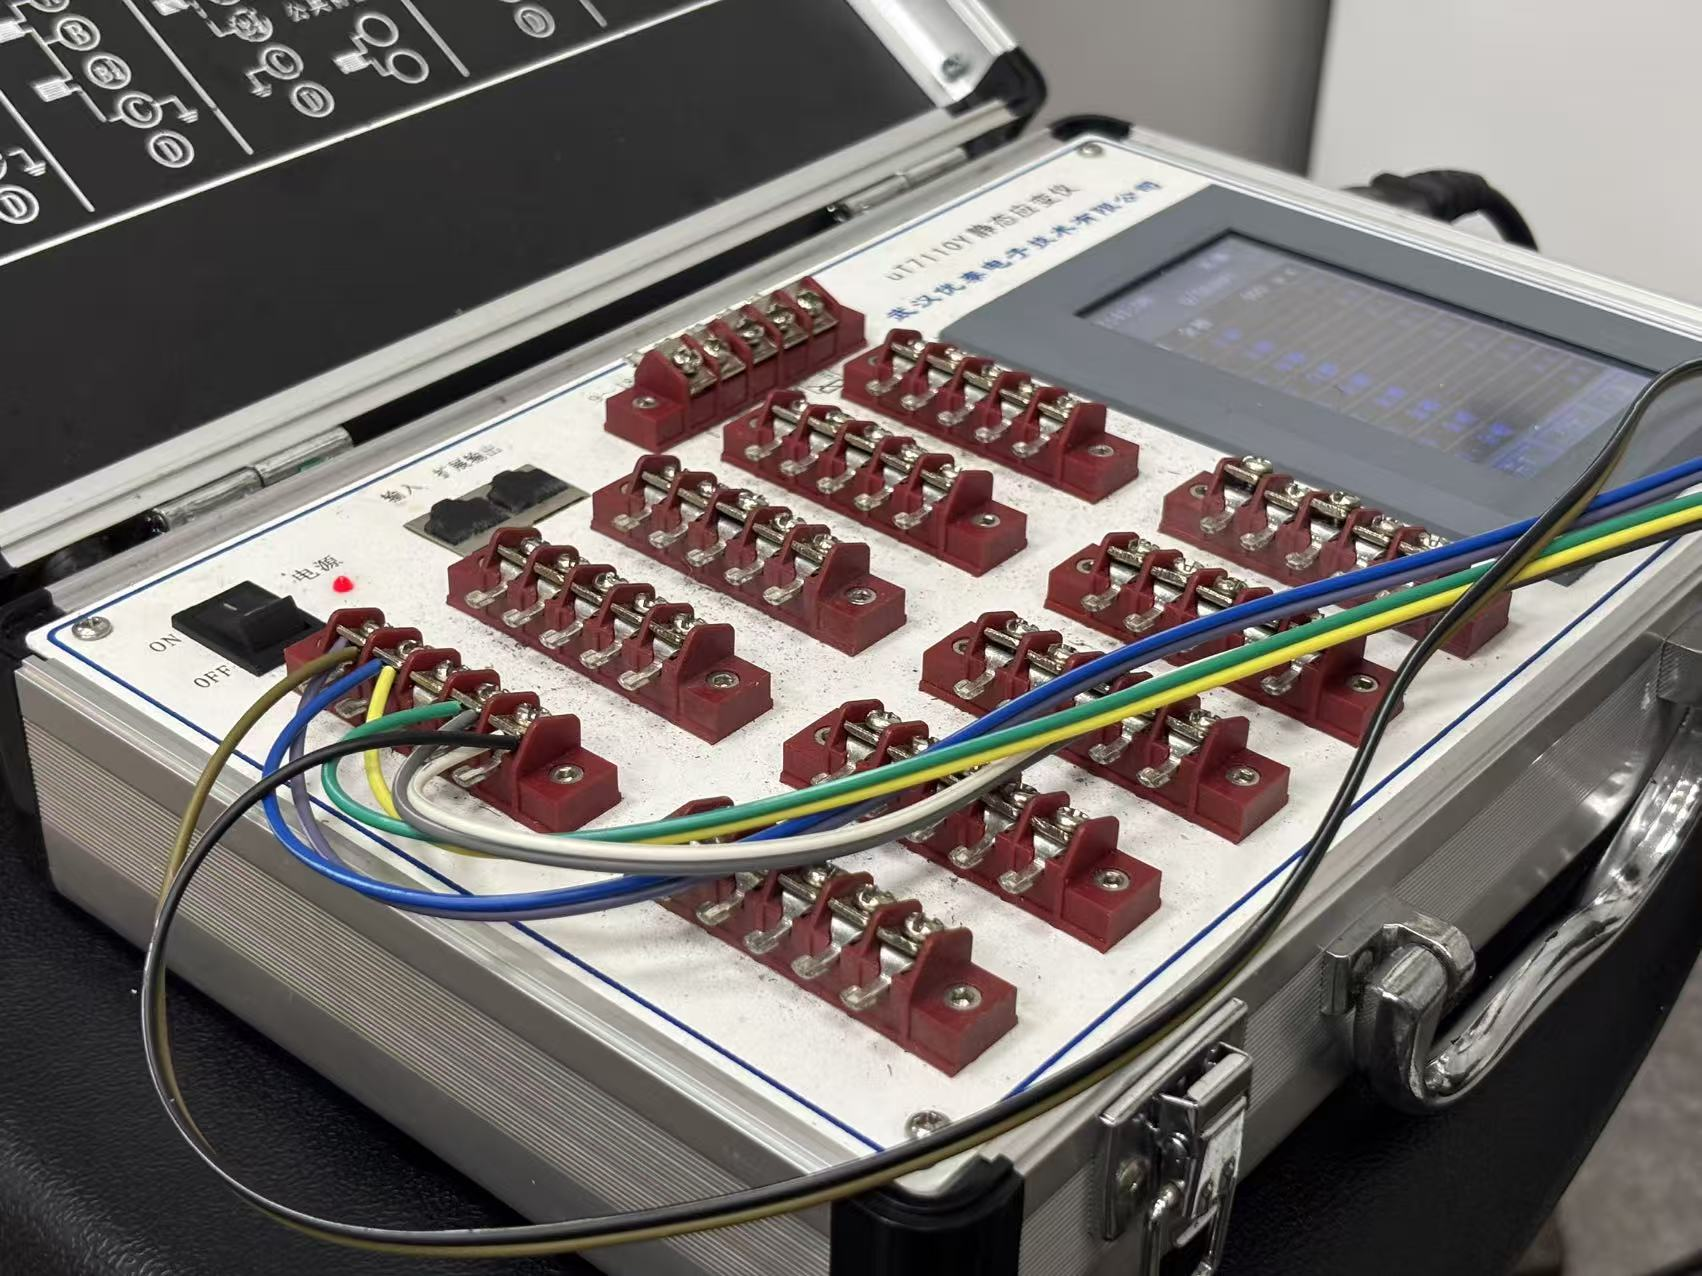
\includegraphics[height=5.2cm]{figures/应变仪.jpg}
    \caption{应变仪}
    \label{fig:strain-instrument}
  \end{subfigure}
  \caption{简易电子秤实验装置实物}
  \label{fig:device-photos}
\end{figure}




\subsection{贴片位置与组桥方案}

根据悬臂梁弯曲理论，梁表面应变在固定端附近较大，但固定端夹持区域存在局部
应力集中和边界约束影响。根据圣维南原理，夹持端引起的局部复杂应力会在离开
端部一定距离后逐渐衰减，因此应变片应布置在距固定端一定距离的位置，并避开
端部约 \(2t\) 的区域。

本实验采用如下方案：
\begin{enumerate}
  \item 在梁上表面和下表面同一截面分别贴片，使其分别处于拉伸和压缩状态；
  \item 沿梁长方向选取两个截面布置应变片，通过差动方式减小加载位置变化对输出
  的影响；同时为削弱固定端局部约束的影响，两个贴片截面坐标分别取
  \(x_1=\SI{40}{mm}\)、\(x_2=\SI{160}{mm}\)；
  \item 贴片位置应尽可能位于对应截面上、下表面的宽度中线上，使应变片主要
  测量由竖向载荷引起的纵向弯曲应变，避免因横向偏移产生附加扭转或局部应变
  差异，从而提高上下表面应变片输出的对称性；
  \item 采用全桥接法提高输出灵敏度，并实现温度补偿；
\end{enumerate}

具体贴片位置与应变符号约定如
表~\ref{tab:gauge-position} 所示。

\begin{table}[htbp]
  \centering
  \begin{tabular}{cp{4.2cm}p{7.6cm}}
    \toprule
    应变片 & 位置 & 应变性质 \\
    \midrule
    \(R_1\) & \(x_1\) 截面上表面中心线 & 位于 \(x_1\) 截面的上表面，按桥路接线符号记为 \(+\varepsilon_1\) \\
    \(R_2\) & \(x_1\) 截面下表面中心线 & 与 \(R_1\) 位于同一截面、相对表面，弯曲应变符号相反，记为 \(-\varepsilon_1\) \\
    \(R_3\) & \(x_2\) 截面下表面中心线 & 位于 \(x_2\) 截面的下表面，与该截面上表面应变符号相反，记为 \(-\varepsilon_2\) \\
    \(R_4\) & \(x_2\) 截面上表面中心线 & 位于 \(x_2\) 截面的上表面，按桥路接线符号记为 \(+\varepsilon_2\) \\
    \bottomrule
  \end{tabular}
  \caption{应变片贴片位置及应变性质}
  \label{tab:gauge-position}
\end{table}



\begin{figure}[htbp]
  \centering
  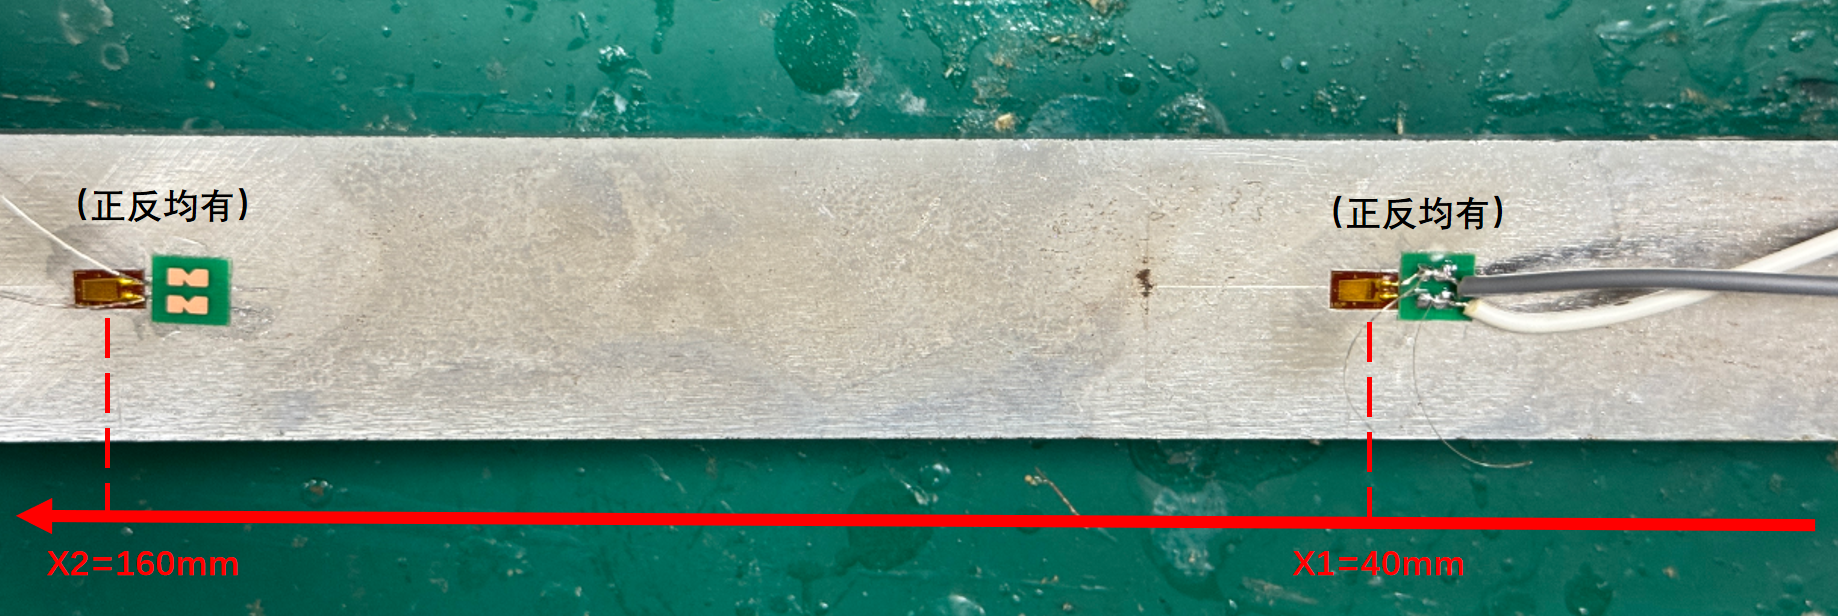
\includegraphics[width=0.8\textwidth]{figures/贴片位置.png}
  \caption{应变片贴片位置与组桥方式示意图}
  \label{fig:gauge-layout}
\end{figure}


上、下表面成对贴片可以将同一截面的拉、压应变同时引入电桥，使弯曲应变信号
相互叠加，从而提高输出灵敏度；对于温度变化或整体轴向拉压引起的均匀电阻变化，
各桥臂变化趋势近似一致，可在差动输出中相互抵消。贴片位置避开梁边缘可以降低
偏心加载时扭转和横向弯曲的影响，保证应变片主要反映竖向载荷引起的纵向弯曲
应变。


\section{强度校核与量程设计}

\subsection{许用应力}

强度校核时安全系数取 \(n=2.5\)，因此许用应力为
\begin{equation}
  [\sigma]=\frac{\sigma_{0.2}}{n}
  =\frac{\SI{980}{MPa}}{2.5}
  =\SI{392}{MPa}.
  \label{eq:allowable-stress}
\end{equation}

\subsection{最大量程估算}

载荷作用于实际挂载位置时，最危险截面位于固定端附近。由
\(\sigma_{\max}=P_{\max}L_1/W\) 可得
\begin{equation}
  P_{\max}=\frac{[\sigma]W}{L_1}.
  \label{eq:max-load}
\end{equation}

由式~\ref{eq:section-modulus} 可得矩形截面的抗弯截面系数为
\begin{equation}
  W=\frac{bt^2}{6}
  =\frac{30\times 4^2}{6}
  =\SI{80}{mm^3}.
  \label{eq:section-modulus-value}
\end{equation}

代入 \([\sigma]=\SI{392}{MPa}=\SI{392}{N/mm^2}\)、\(W=\SI{80}{mm^3}\)
和 \(L_1=\SI{320}{mm}\)，可得
\begin{equation}
  P_{\max}
  =\frac{[\sigma]W}{L_1}
  =\frac{392\times 80}{320}
  =\SI{98}{N}.
  \label{eq:max-load-value}
\end{equation}

取重力加速度 \(g=\SI{9.81}{m/s^2}\)，对应理论最大质量为
\begin{equation}
  m_{\max}=\frac{P_{\max}}{g}
  =\frac{98}{9.81}
  =\SI{9.99}{kg}\approx \SI{10.0}{kg}.
  \label{eq:max-mass}
\end{equation}
因此，在所取安全系数下，弹性元件的理论最大量程约为 \(\SI{10.0}{kg}\)。

需要说明的是，上述 \(\SI{10.0}{kg}\) 是由强度条件得到的理论承载上限，主要
用于判断弹性元件在极限工作状态下是否满足安全要求，并不等同于最终采用的
实验有效量程。本实验标定数据最高覆盖至
\(\SI{8.0}{kg}\)，且高载荷下梁挠度和加载平台转角进一步增大，因此后续数据处理
与精度评价均以 \(0\sim\SI{8.0}{kg}\) 作为电子秤的实际有效量程。


标定前在设计量程最大值附近进行 2--3 次预加载，以确认弹性元件无永久变形、
应变输出稳定，且电路输出未超过仪表量程。

\section{实验方法}

\subsection{实验步骤}

\begin{enumerate}
  \item 对梁表面进行打磨、清洁、定位和贴片；
  \item 焊接引线并完成电桥组桥；
  \item 安装梁和加载平台，完成电路平衡；
  \item 在设计最大量程附近预加载 2--3 次；
  \item 按 6 个加载点逐级加载，记录质量和输出信号，卸载并重复加载实验2次并记录数据，取三次测量的平均值；
  \item 对得到的$m-\epsilon$数据进行线性拟合，得到并修改灵敏度参数，完成传感器的标定；
  \item 按 6 个加载点逐级加载（选取重量数值不应与标定时相同），记录质量和输出信号，卸载并重复加载实验2次并记录数据，取三次测量的平均值；
  \item 对数据进行误差分析和精度等级评价。
\end{enumerate}

\section{数据处理}

\subsection{数据记录表}

\begin{table}[H]
  \centering
  \begin{tabular}{ccccc}
    \toprule
    质量 \(m\)/kg & 标定读数 1 & 标定读数 2 & 标定读数 3 & 平均读数 \\
    \midrule
    0.0 & 3 & -1 & 0 & 0.67 \\
    1.5 & 235 & 233 & 230 & 232.67 \\
    3.0 & 465 & 450 & 459 & 458.00 \\
    4.5 & 693 & 672 & 695 & 686.67 \\
    6.0 & 928 & 906 & 923 & 919.00 \\
    7.0 & 1053 & 1049 & 1055 & 1052.33 \\
    8.0 & 1203 & 1205 & 1204 & 1204.00 \\
    \bottomrule
  \end{tabular}
  \caption{标定实验原始数据}
  \label{tab:calibration-raw-data}
\end{table}

标定时，应变仪中的灵敏度参数初始设置为 \(S_0=2.00\)。由表
\ref{tab:calibration-raw-data} 中三次标定读数的平均值进行线性拟合，得到斜率
\(k=150.4191\)，即应变仪读数随加载质量的变化率为
\(\SI{150.4191}{kg^{-1}}\)。为使应变仪显示值直接对应加载质量，目标斜率取
\(k_{\mathrm{t}}=1.0000\)。由于应变仪显示读数与灵敏度设置值近似成反比，修改后的
灵敏度参数应满足
\begin{equation}
  S_{\mathrm{new}}
  =S_0\frac{k}{k_{\mathrm{t}}}
  =2.00\times 150.4191
  =300.8382.
  \label{eq:instrument-sensitivity-setting}
\end{equation}
因此，标定完成后将应变仪灵敏度参数由 \(2.00\) 调整为约 \(300.84\)，并重新调零
以消除零点偏置的影响。

\begin{table}[htbp]
  \centering
  \begin{tabular}{ccccc}
    \toprule
    质量 \(m\)/kg & 升载读数 1 & 升载读数 2 & 升载读数 3 & 平均读数 \\
    \midrule
    0.0 & 0 & 0 & 0 & 0.00 \\
    1.0 & 1.0 & 1.0 & 1.0 & 1.00 \\
    2.0 & 2.0 & 2.0 & 2.0 & 2.00 \\
    4.0 & 4.0 & 4.0 & 4.1 & 4.03 \\
    5.0 & 5.1 & 5.1 & 5.1 & 5.10 \\
    6.5 & 6.5 & 6.6 & 6.4 & 6.50 \\
    7.5 & 7.6 & 7.6 & 7.6 & 7.60 \\
    \bottomrule
  \end{tabular}
  \caption{升载测试实验原始数据}
  \label{tab:test-raw-data}
\end{table}

为进一步检查加载历史对应变仪显示值的影响，测试阶段还记录了卸载过程中的读数。
卸载数据如表~\ref{tab:unload-raw-data} 所示。

\begin{table}[htbp]
  \centering
  \begin{tabular}{cc}
    \toprule
    标准质量 \(m\)/kg & 卸载读数/kg \\
    0.0 & 0.0  \\
    1.0 & 1.1  \\
    2.0 & 2.0  \\
    4.0 & 4.1  \\
    5.0 & 5.0  \\
    6.5 & 6.6  \\
    7.5 & 7.6  \\
    \bottomrule
  \end{tabular}
  \caption{卸载测试实验数据}
  \label{tab:unload-raw-data}
\end{table}

\subsection{质量--输出关系拟合}

将标定数据按线性模型进行拟合：
\begin{equation}
  U_{\mathrm{amp}} = k m + b,
  \label{eq:linear-fit}
\end{equation}
其中 \(k\) 为灵敏度，\(b\) 为零点偏置。由最小二乘法得到拟合直线后，可进一步
计算各测点的残差：
\begin{equation}
  \delta_i = U_i - (k m_i+b).
  \label{eq:residual}
\end{equation}

对三次标定读数取平均值后进行线性拟合，得到标定关系为
\begin{equation}
  y=150.4191m+5.8230,
  \label{eq:calibration-result}
\end{equation}
其中 \(m\) 为加载质量，单位为 kg，\(y\) 为应变仪读数。拟合决定系数为
\(R^2=0.99981\)，表明输出读数与加载质量之间具有良好的线性关系。

\begin{figure}[htbp]
  \centering
  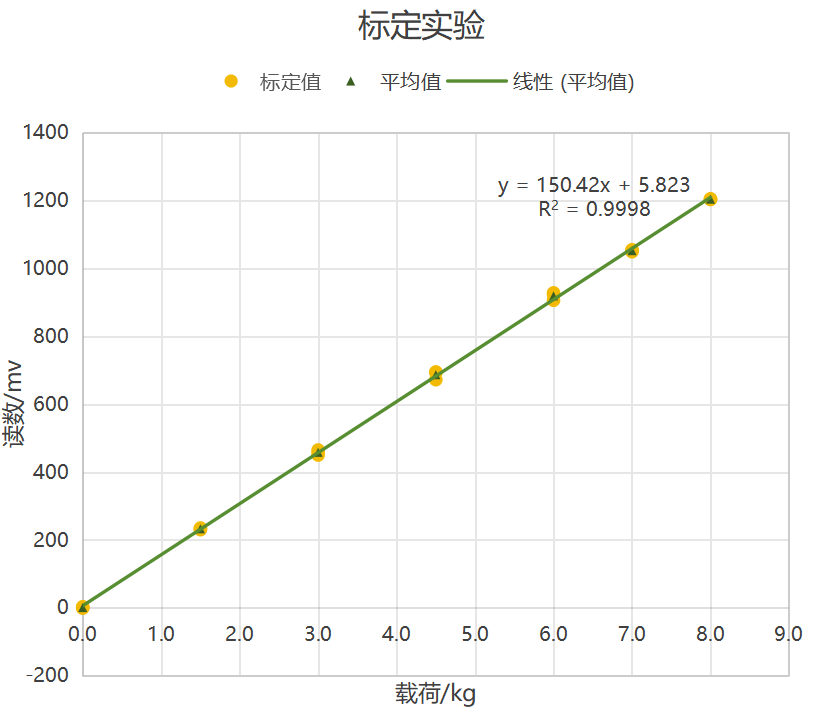
\includegraphics[width=0.70\textwidth]{figures/标定实验.png}
  \caption{标定曲线及线性拟合结果}
  \label{fig:calibration}
\end{figure}

应变仪灵敏度参数修正后，进一步利用测试实验数据检验电子秤的实际显示效果。
测试数据不参与灵敏度参数的确定，而用于评价标定后仪器显示值与真实加载质量的
一致性。将测试阶段的平均显示值与实际加载质量进行线性拟合，得到
\begin{equation}
  m_{\mathrm{display}}=1.0054m+0.0086,
  \label{eq:test-fit}
\end{equation}
拟合决定系数为 \(R^2=0.99984\)。该结果表明，标定后的电子秤显示值与实际质量
基本呈一一对应关系，整体线性较好。

\begin{figure}[htbp]
  \centering
  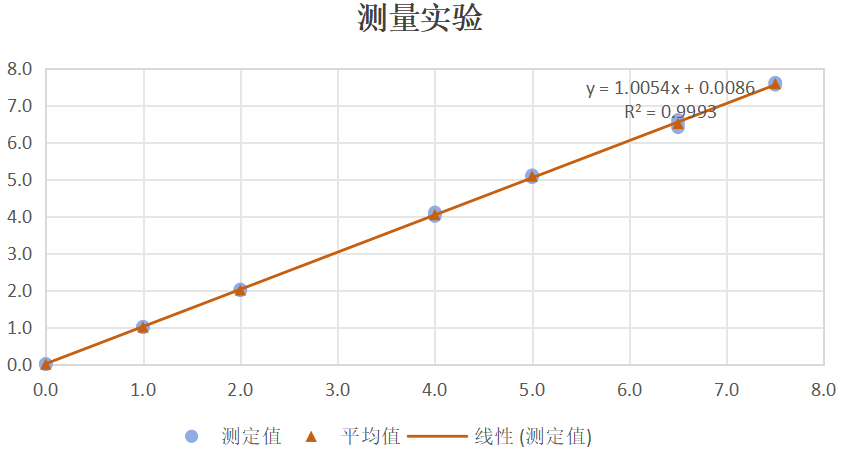
\includegraphics[width=0.70\textwidth]{figures/测量实验.png}
  \caption{测量曲线及线性拟合结果}
  \label{fig:test-fit}
\end{figure}

由图~\ref{fig:test-fit} 可见，各测试点基本分布在理想线性关系附近。与标定曲线
相比，测量曲线更直接反映灵敏度修正后的称量效果：在 \(0\sim\SI{7.5}{kg}\) 的
测试范围内，显示值随加载质量近似线性增加，最大示值偏差为 \(\SI{0.10}{kg}\)。

\subsection{灵敏度、线性度与有效量程}

由标定曲线可知，初始设置下电子秤的输出灵敏度为
\(S=\SI{150.4191}{kg^{-1}}\)，表示应变仪读数随加载质量的变化率。

误差计算取有效满量程 \(m_{\mathrm{FS}}=\SI{8.0}{kg}\)。由标定与测试数据可得，
主要误差指标汇总见表~\ref{tab:error-summary}。

\begin{figure}[htbp]
  \centering
  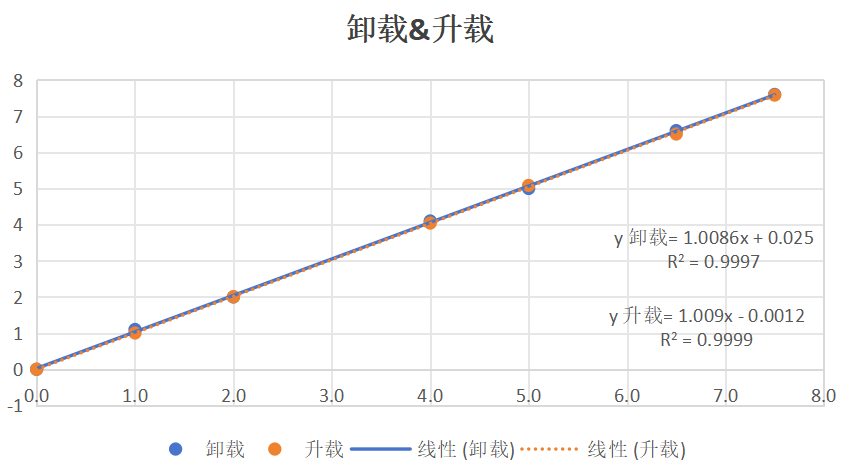
\includegraphics[width=0.70\textwidth]{figures/升载卸载曲线.png}
  \caption{升载与卸载测试结果对比}
  \label{fig:loading-unloading}
\end{figure}

由图~\ref{fig:loading-unloading} 可见，升载和卸载结果整体接近，个别测点存在
小幅回程差。

\begin{table}[htbp]
  \centering
  \begin{tabular}{ccc}
    \toprule
    误差指标 & 数值 & 主要反映内容 \\
    \midrule
    线性度误差 \(e_L\) & \(0.886\%\) & 标定点相对拟合直线的偏离 \\
    重复度误差 \(e_R\) & \(1.911\%\) & 同一载荷重复读数的离散程度 \\
    满量程引用误差 \(\gamma\) & \(1.25\%\) & 测试示值相对满量程的偏差 \\
    回程误差 \(e_H\) & \(1.25\%\) & 升载与卸载读数的差异 \\
    \bottomrule
  \end{tabular}
  \caption{电子秤主要误差指标汇总}
  \label{tab:error-summary}
\end{table}

取四项误差中的最大值作为控制性误差：
\begin{equation}
  e_{\mathrm{c}}
  =\max(e_L,e_R,\gamma,e_H)
  =\max(0.886\%,1.911\%,1.25\%,1.25\%)
  =1.911\%.
  \label{eq:combined-error}
\end{equation}
据此可将精度等级定为 \(2\) 级。

\section{误差分析}

本实验误差主要来自四方面：一是固定端夹持并非理想固支，夹具变形会改变有效力臂和零点；二是砝码放置偏心、高载荷挠度较大，带来附加扭转和几何非线性；三是应变片贴片位置、粘贴质量及温度漂移影响电桥输出；四是读数时机、振动和升卸载迟滞造成随机离散。改进时应保证加载居中，充分预加载，待读数稳定后记录，并优化夹具刚度和贴片对称性。

\section{结论}

本文完成了悬臂梁式简易电子秤的弹性元件设计、应变片布置、全桥组桥、标定
与精度评价。应变片沿梁长方向布置在两个截面，并尽量位于上、下
表面宽度中线处，通过全桥接法提高输出灵敏度并减小温度变化对测量结果的影响。

强度校核结果表明，在安全系数 \(n=2.5\) 下，许用应力为
\([\sigma]=\SI{392}{MPa}\)，由矩形截面抗弯截面系数
\(W=\SI{80}{mm^3}\) 计算得到理论最大载荷为 \(P_{\max}=\SI{98}{N}\)，
对应理论最大质量约为 \(\SI{10.0}{kg}\)。考虑实验加载条件、读数稳定性和标定
数据范围，本文将电子秤实际有效量程取为 \(0\sim\SI{8.0}{kg}\)。

标定实验结果显示，应变仪读数与加载质量之间具有较好的线性关系，拟合方程为
\(y=150.4191m+5.8230\)，决定系数为 \(R^2=0.99981\)。根据该斜率对
应变仪灵敏度参数进行修正后，
按 \(\SI{8.0}{kg}\) 满量程计算的引用误差为 \(1.25\%\)。综合线性度误差
\(0.886\%\)、重复度误差 \(1.911\%\)、满量程引用误差 \(1.25\%\) 和回程误差
\(1.25\%\)，控制性误差为 \(1.911\%\)，因此本实验制作的简易电子秤按常用精度
等级可定为约 \(2\) 级。

实验误差主要来源于固定端夹持条件与理想悬臂梁模型的差异、应变片贴片位置偏差、
加载偏心、桥路零点漂移以及应变仪读数分辨率等。后续可通过提高夹具刚度、优化
加载平台导向结构、改进贴片定位精度、增加重复测量次数和进行温度补偿等方式，
进一步提高电子秤的稳定性和测量精度。

\section{实验心得}

本次实验又小组成员齐心协力共同完成，期间遇到过一些问题当然最后也成功地解决了，让我们对材料力学和传感器制作有了更深的理解。
最大的体会是，简易电子秤的精度并不仅由理论计算决定，实际装配和调试
过程对结果影响很明显。实验初期，应变仪读数存在较明显的零点偏移，而且偏移量
会随时间逐渐增大。起初我们主要从电桥平衡和仪器调零角度排查，后来发现接线端
螺丝没有完全拧紧，导线接触状态不稳定会使桥路电阻发生微小变化，从而造成读数
缓慢漂移。将接线螺丝重新拧紧后，零点稳定性明显改善。

贴片和引线保护也是实验中比较容易忽视的问题。应变片贴好后，由于引线较细，在
移动梁或整理线路时曾出现贴片被拉动甚至脱落的情况。后续我们用电工胶布对导线
进行固定和缓冲，这样就不容易掉落了。这个过程让我们认识到，应变片本身虽然很小，但贴片质量、焊点保护和
导线走向都会直接影响测量稳定性。

从理论计算到实际贴片和实验，这一过程真正将课堂上学到的东西运用到了实际，收获很大。


\begin{figure}[H]
  \centering
  % 第一张图
  \begin{subfigure}[b]{0.31\textwidth}
    \centering
    % 建议把 height 换成 width=\textwidth，让图片自动适应子图的宽度
    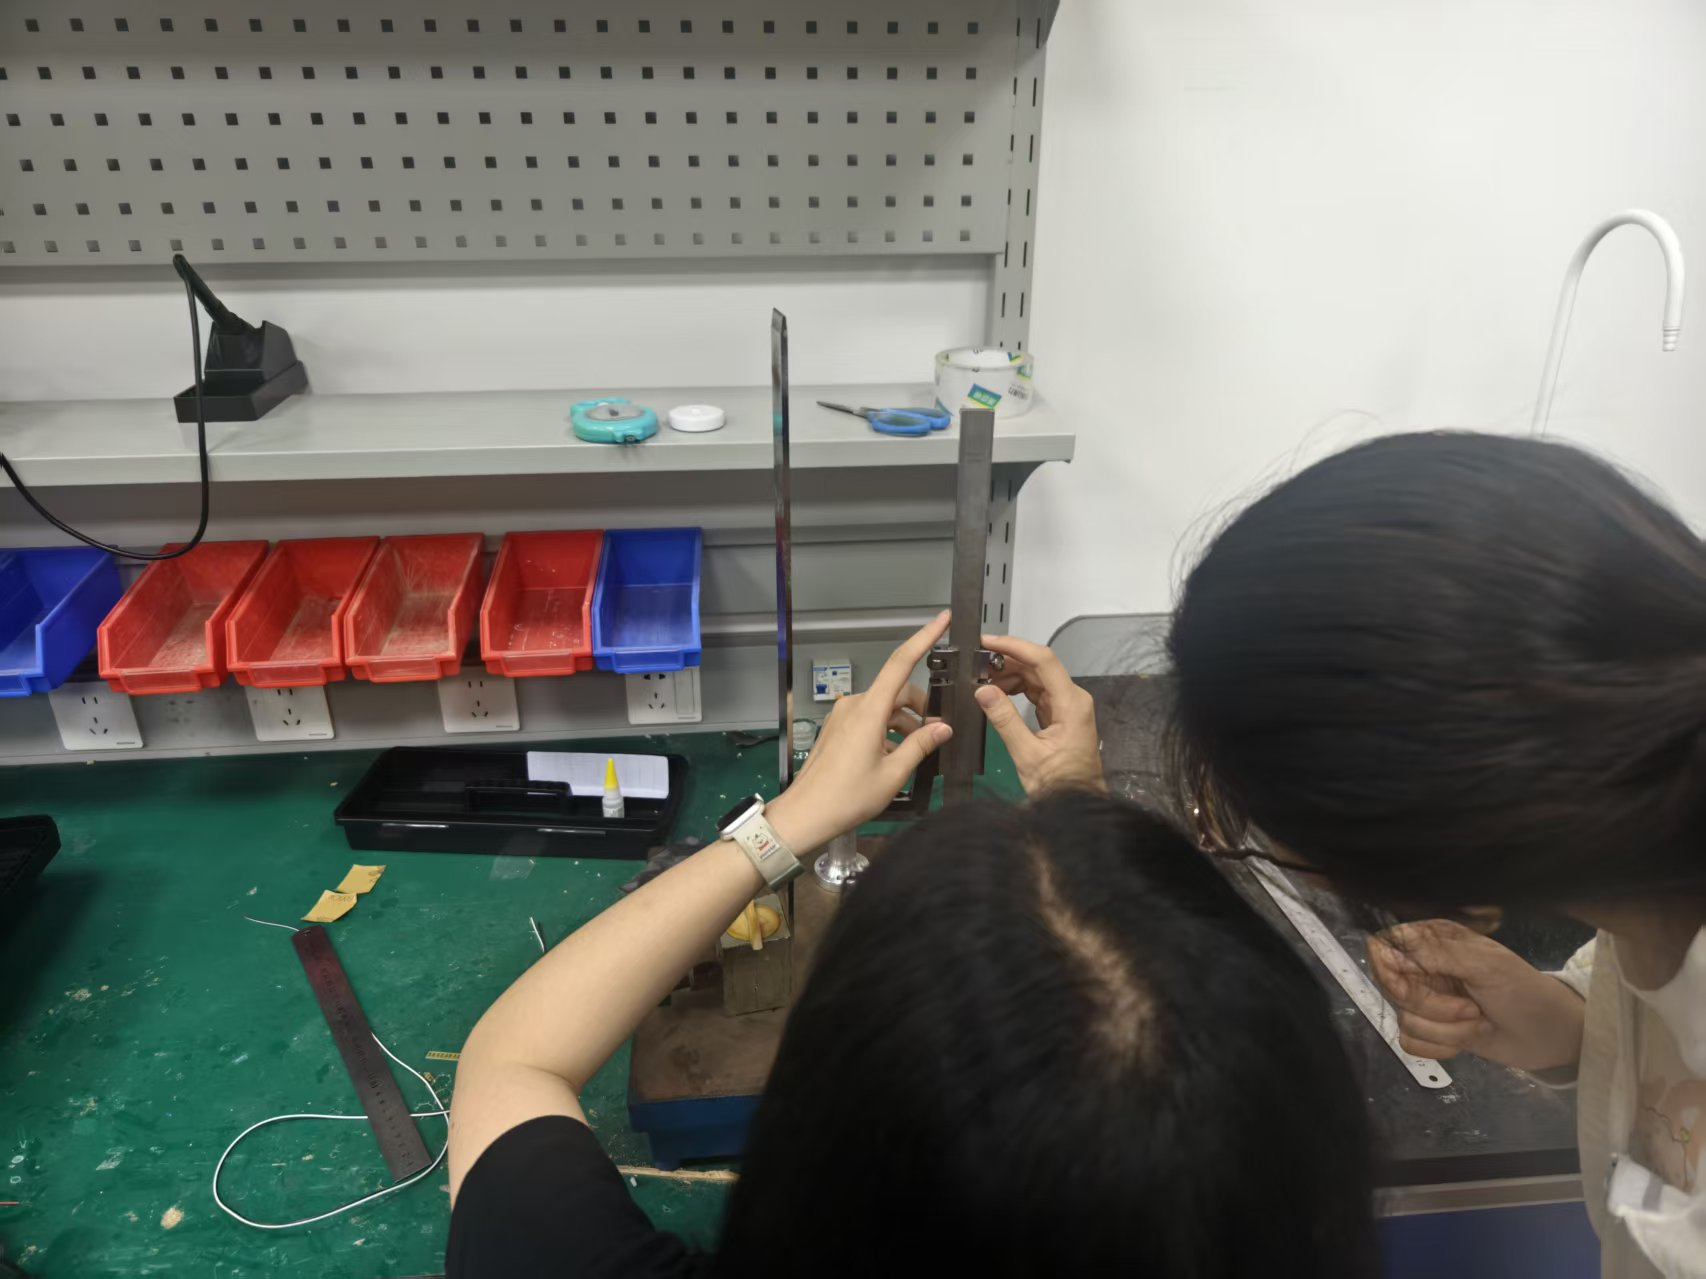
\includegraphics[width=\textwidth]{figures/划线.jpg}
    \caption{在试样上划线}
    \label{fig:process-marking}
  \end{subfigure}
  \hfill % 自动在一二图之间插入弹性空白
  % 第二张图
  \begin{subfigure}[b]{0.31\textwidth}
    \centering
    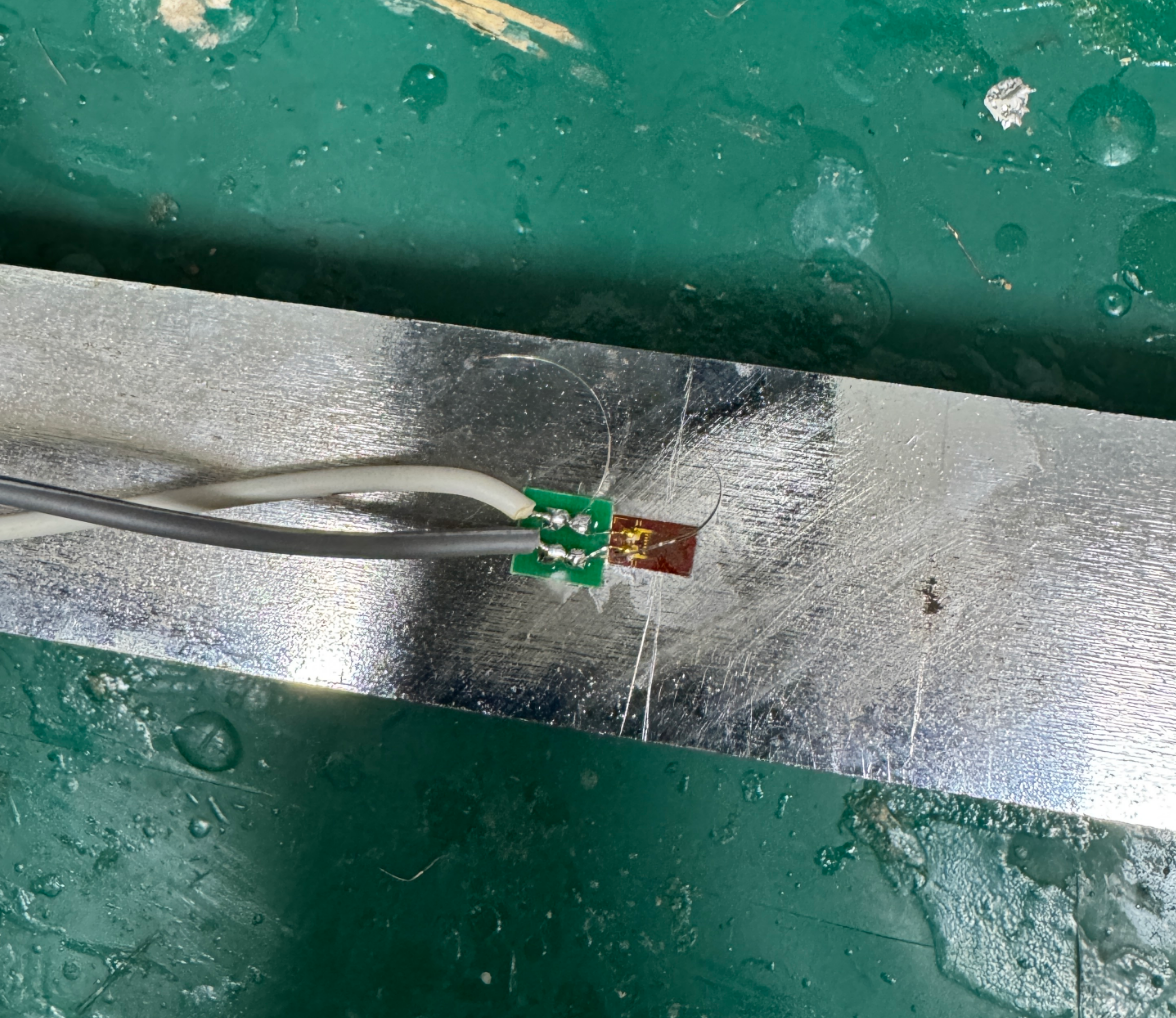
\includegraphics[width=\textwidth]{figures/贴片.png}
    \caption{贴应变片}
    \label{fig:process-gauge-bonding}
  \end{subfigure}
  \hfill % 自动在二三图之间插入弹性空白
  % 第三张图
  \begin{subfigure}[b]{0.31\textwidth}
    \centering
    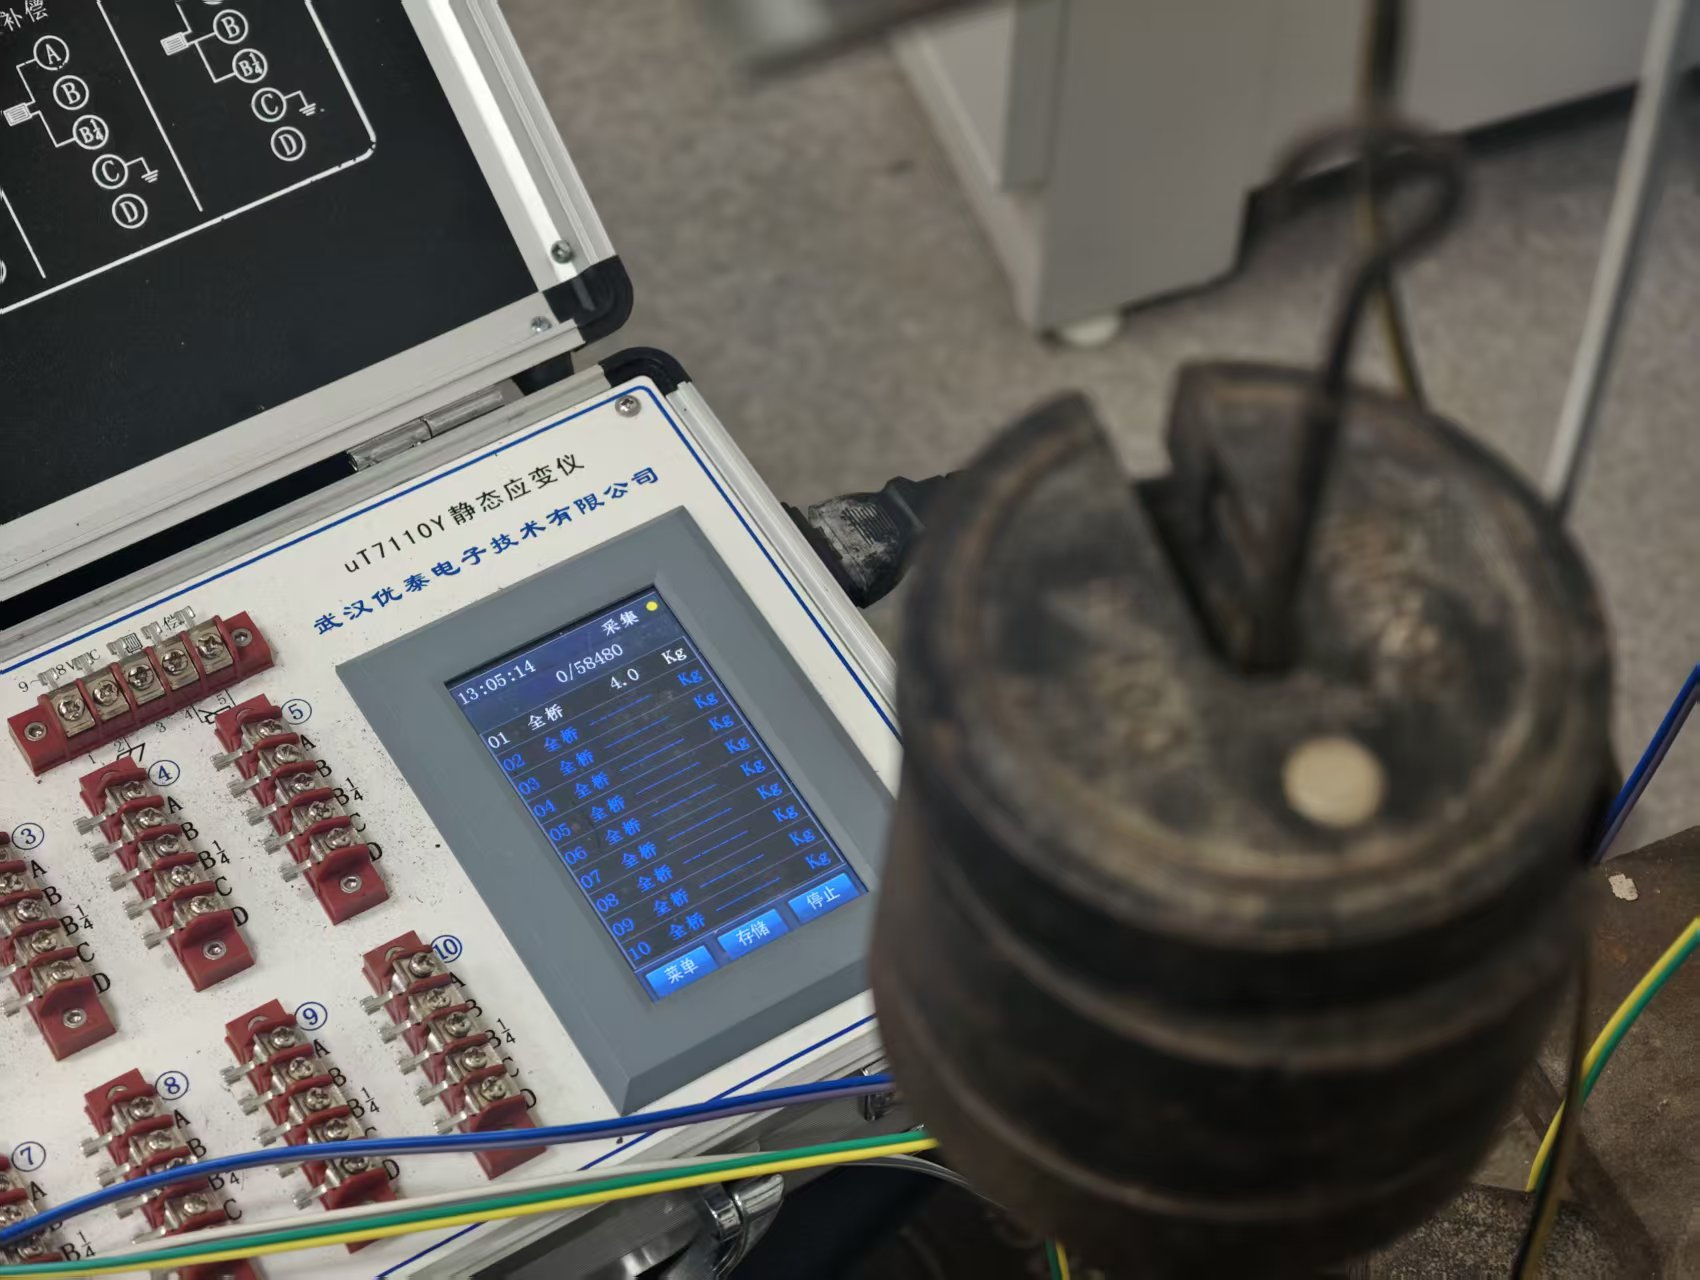
\includegraphics[width=\textwidth]{figures/测量.jpg} % 请替换为你的第三张图路径
    \caption{标定后测量} % 请替换为你的第三张图标题
    \label{fig:weights}
  \end{subfigure}
  
  \caption{制作过程记录}
  \label{fig:process-record}
\end{figure}



\section{小组成员分工}

本实验由小组成员协作完成，各成员在方案设计、装置制作、实验测试和论文整理中
均有参与。具体分工如表~\ref{tab:team-work} 所示。

\begin{table}[htbp]
  \centering
  \begin{tabular}{cp{10.5cm}}
    \toprule
    成员 & 主要分工 \\
    \midrule
    韩颂义 & 负责实验方案总体设计、悬臂梁受力分析、强度校核与量程估算、论文结构整理和最终答辩展示 \\
    姚珂尔 & 负责应变片贴片、桥路连接与应变仪调试，参与加载实验和原始数据记录以及答辩PPT的制作 \\
    张雨童 & 负责标定实验与测试实验的数据采集、数据表格整理、标定曲线绘制和误差分析 \\
    \bottomrule
  \end{tabular}
  \caption{小组成员分工}
  \label{tab:team-work}
\end{table}

\section{致谢}

感谢王双连、雷华老师在实验方案设计、应变片贴片、桥路连接和数据标定过程
中给予的指导。感谢实验室提供的试验设备、应变仪和加载装置，使本实验能够顺利
完成。同时感谢小组成员在弹性元件制作、实验调试、数据记录和论文整理过程中的
分工协作。

\begin{thebibliography}{9}
  \bibitem{materials-mechanics}
  刘鸿文. 材料力学. 北京: 高等教育出版社.

  \bibitem{lab-manual}
  浙江大学材料力学实验指导资料. 悬臂梁式简易电子秤任务书.
\end{thebibliography}




\end{document}
